\documentclass[aspectratio=169]{beamer}
%
% Choose how your presentation looks.
%
% For more themes, color themes and font themes, see:
% http://deic.uab.es/~iblanes/beamer_gallery/index_by_theme.html
%
\mode<presentation>
{
  \usetheme{metropolis}      % or try Darmstadt, Madrid, Warsaw, ...
  \usecolortheme{metropolis-imagelab} % or try albatross, beaver, crane, ...
  \usefonttheme{structurebold}  % or try serif, structurebold, ...
  \setbeamercolor{background canvas}{bg=white}
  \setbeamertemplate{navigation symbols}{}
  \setbeamertemplate{bibliography item}{\insertbiblabel}
  %\setbeamertemplate{caption}[numbered]
} 
\usepackage[english]{babel}
\usepackage[utf8x]{inputenc}
\usepackage{listings}             % Include the listings-package
\hypersetup{
    colorlinks = true,
    linkcolor = {black},
    urlcolor = {blue}
}
\usepackage{animate}

\DeclareMathOperator*{\argmin}{arg\,min}

\title[Unsupervised learning: Clustering]{Unsupervised learning: Clustering}
\subtitle{Pattern Recognition and Machine Learning - 2017}
\institute{University of Modena and Reggio Emilia}
\author{Davide Abati}
\date{September 28th, 2017}

\def\thisframelogos{}

\newcommand{\framelogo}[1]{\def\thisframelogos{#1}}

\begin{document}

\framelogo{logo_unimore_white.png}

\bgroup
\renewcommand{\insertframenumber}{}
\begin{frame}[noframenumbering]
  \titlepage
\end{frame}
\egroup
\begin{frame}{Agenda}
  \tableofcontents
\end{frame}


\section{K-means}
\begin{frame}{K-means}
\begin{itemize}
\item Is a partitional clustering model
\begin{itemize}
\item splits data $\{x_i\}_1^n$ into $k$ disjoint sets
\item the number of sets $k$ has to be provided as input
\end{itemize}
\item solves the following optimization problem:
\begin{align*}
\argmin_{\{c_1, \ldots, c_k\}} = \sum_{j=1}^k\sum_{i=1}^n \mathbf{I}(i,j)||x_i - c_j ||^2 
\end{align*}
\begin{align*}
\mathbf{I}(i,j)=
\begin{cases}
    1, & \text{$x_i$ belongs to cluster $j$}\\
    0,              & \text{otherwise}
\end{cases}
\end{align*}
\end{itemize}
\end{frame}
\begin{frame}{K-means: algorithm}
The problem is NP-hard. A simple heuristic algorithm can be employed to converge to a \emph{local} minimum:
\begin{itemize}
\item Initialize $k$ centers randomly
\item Repeat until convergence:
\begin{itemize}
\item assign each example to the closest center (i.e. lower euclidean distance)
\item re-estimate centers as the mean of their clusters
\end{itemize}
\end{itemize}
Try to implement it from scratch!
\end{frame}
%\bgroup
%\begin{frame}{K-means: iterations}
%\setlength{\tabcolsep}{.07em}
%\begin{figure}
%\begin{tabular}{cccc}
%\small{it 1} & \small{it 2} & \small{it 3} & \small{it 4}\\
%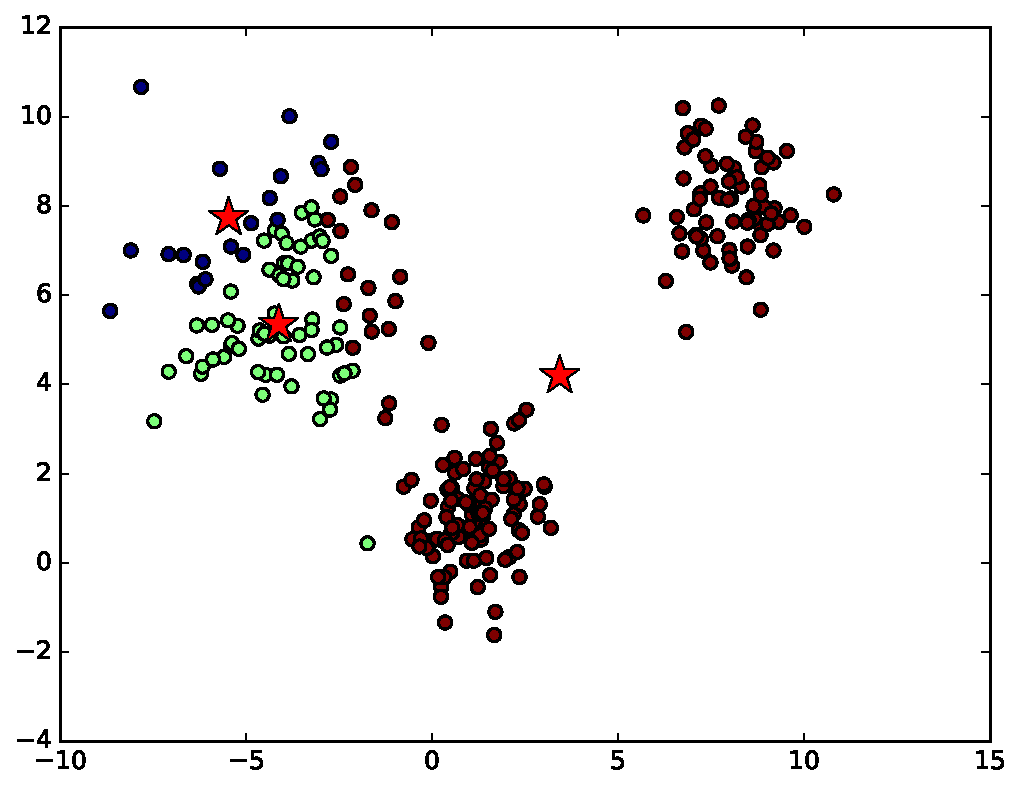
\includegraphics[width=0.25\textwidth]{img/kmeans/it01.pdf}&
%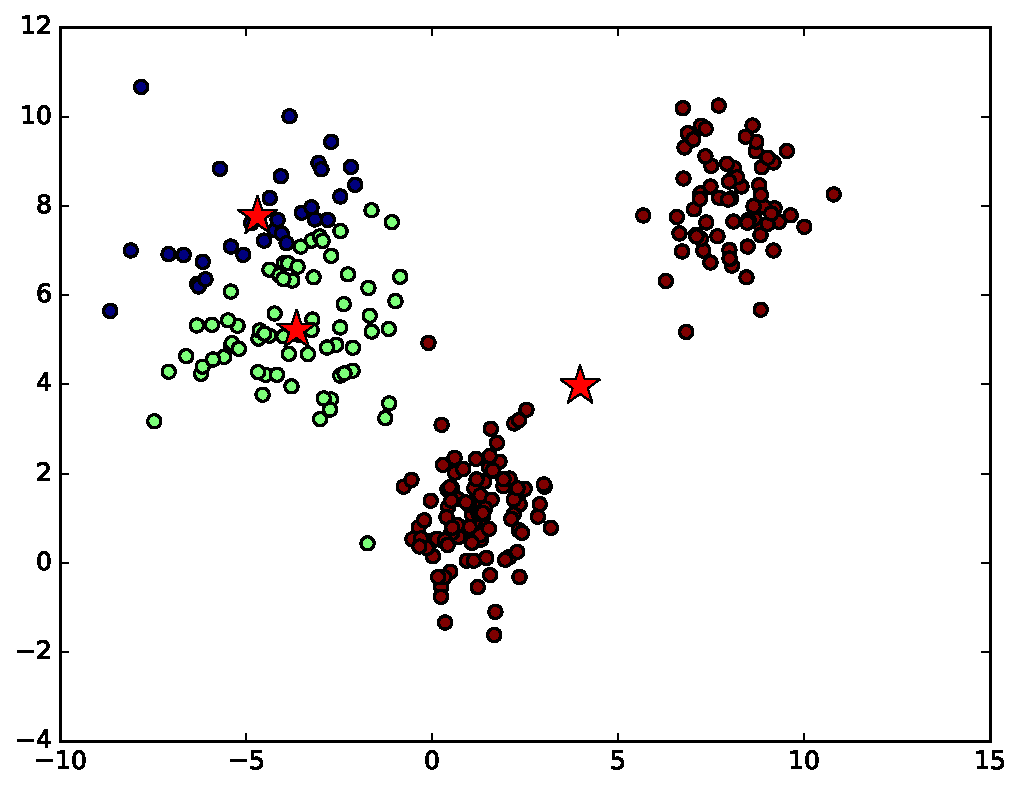
\includegraphics[width=0.25\textwidth]{img/kmeans/it02.pdf}&
%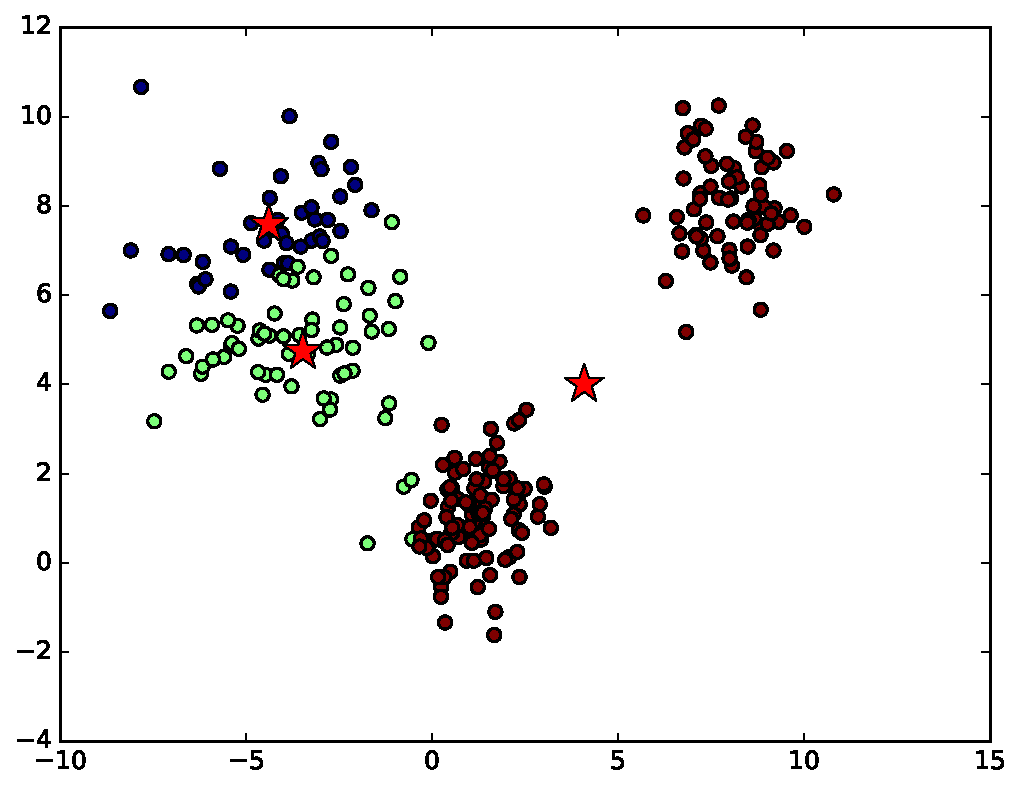
\includegraphics[width=0.25\textwidth]{img/kmeans/it03.pdf}&
%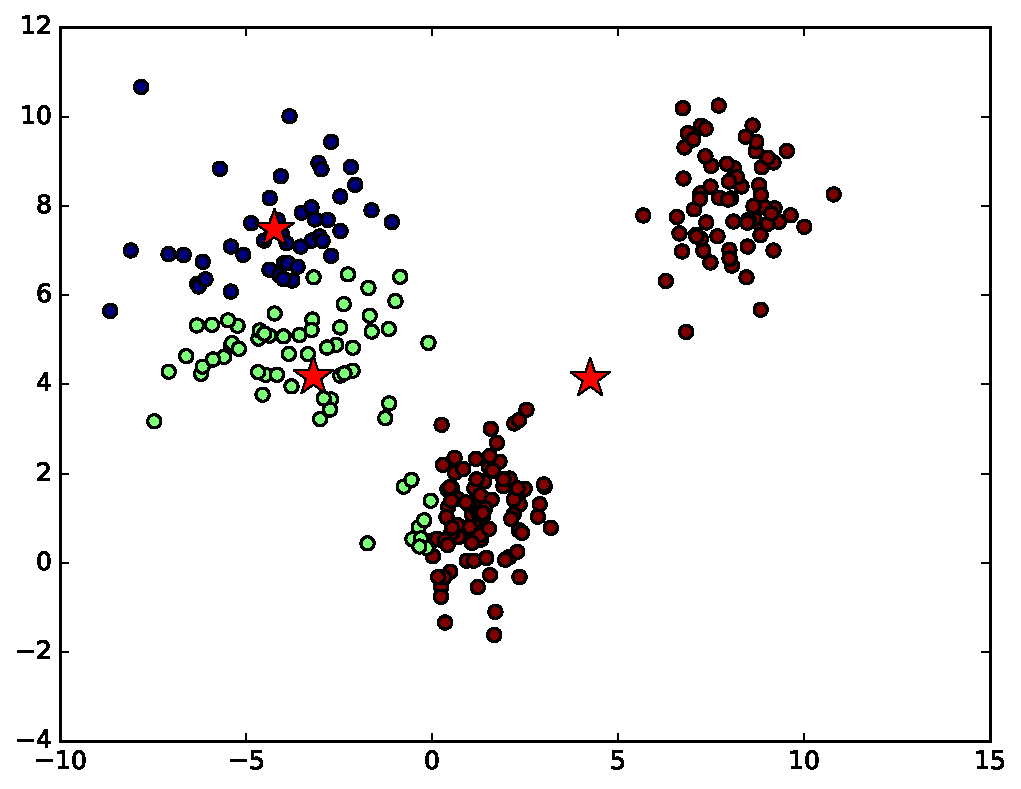
\includegraphics[width=0.25\textwidth]{img/kmeans/it04.pdf}\\
%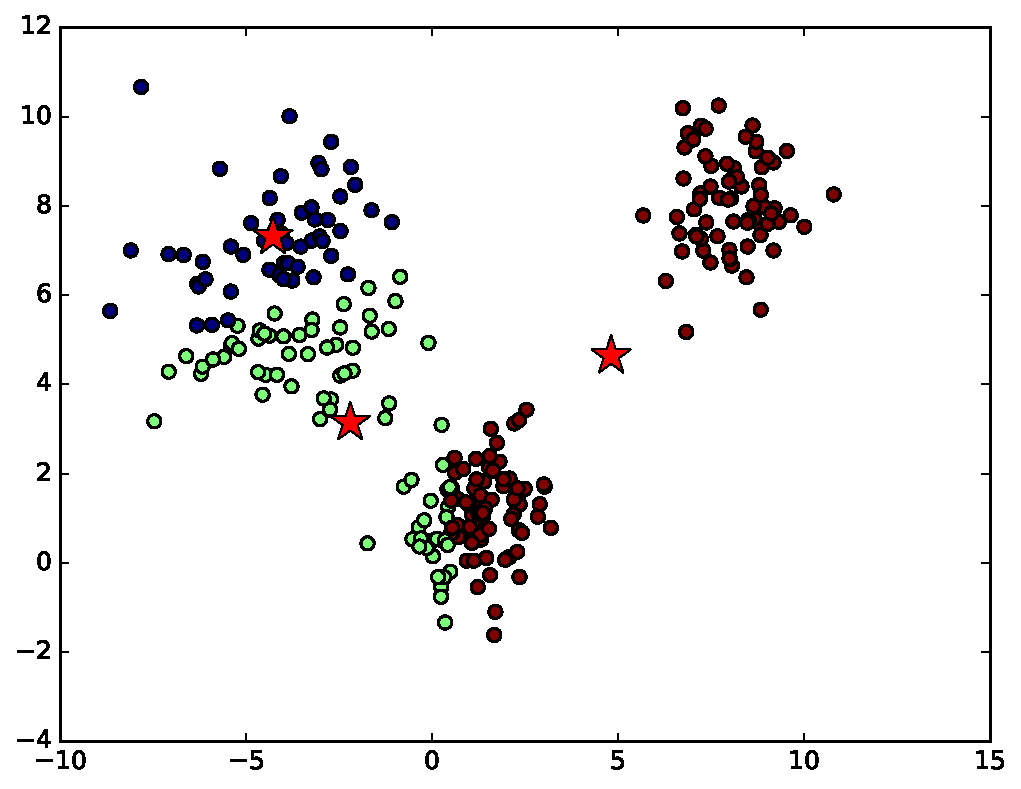
\includegraphics[width=0.25\textwidth]{img/kmeans/it05.pdf}&
%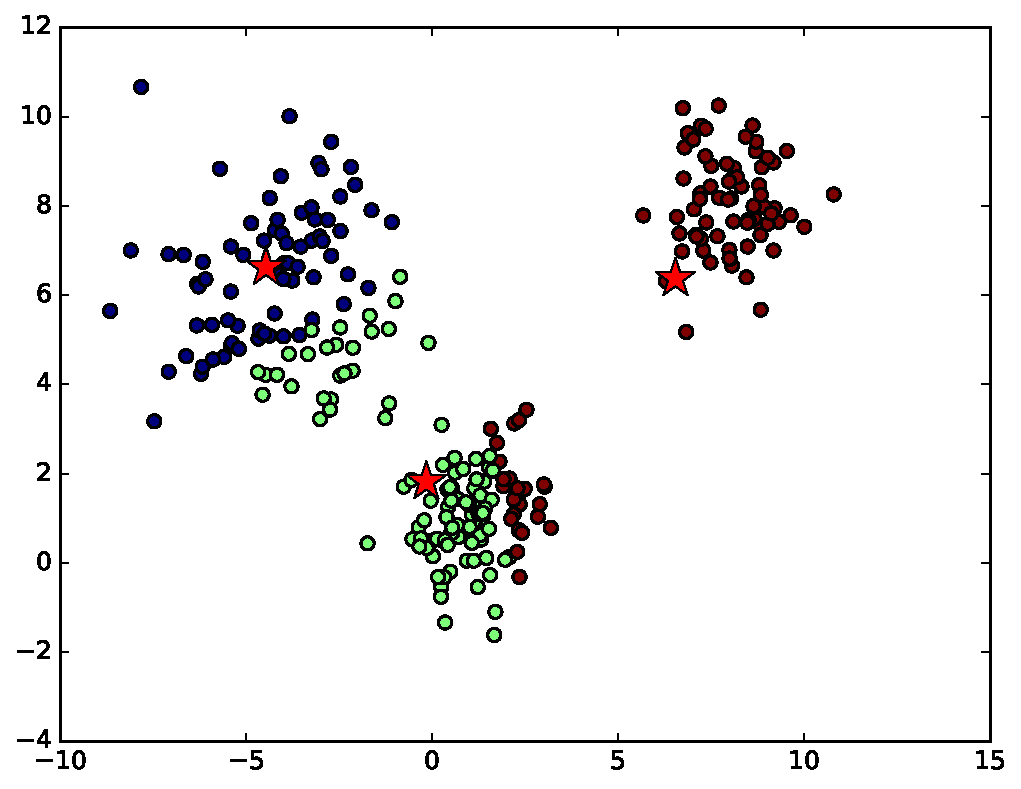
\includegraphics[width=0.25\textwidth]{img/kmeans/it06.pdf}&
%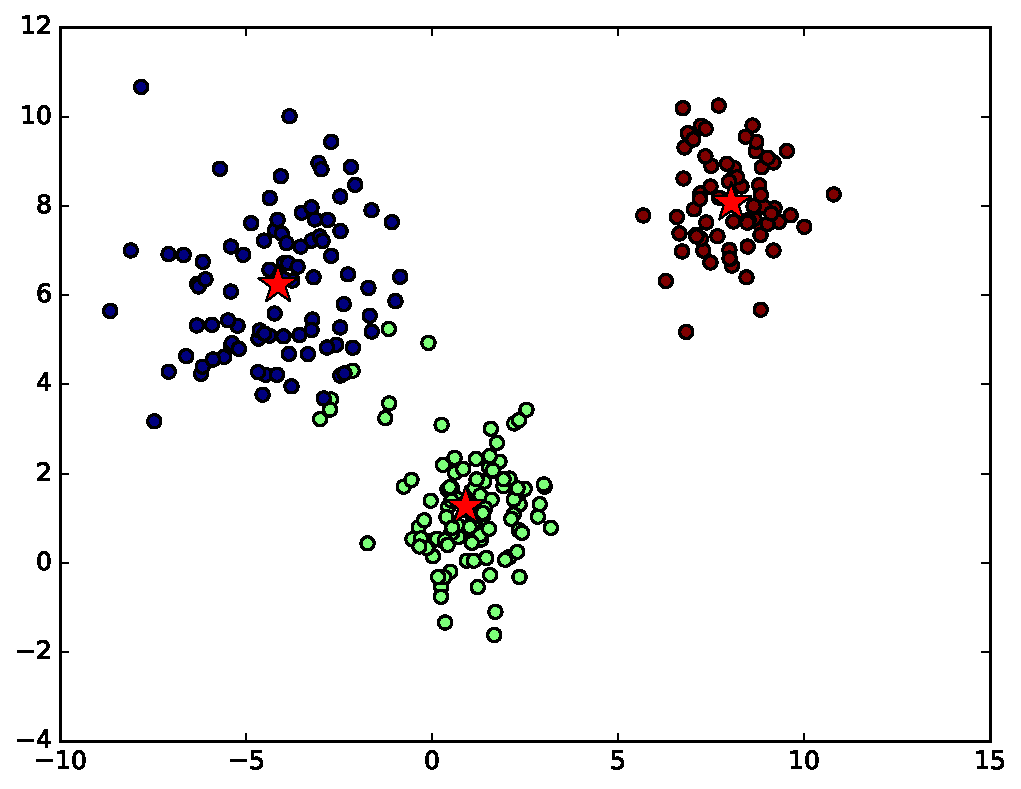
\includegraphics[width=0.25\textwidth]{img/kmeans/it07.pdf}&
%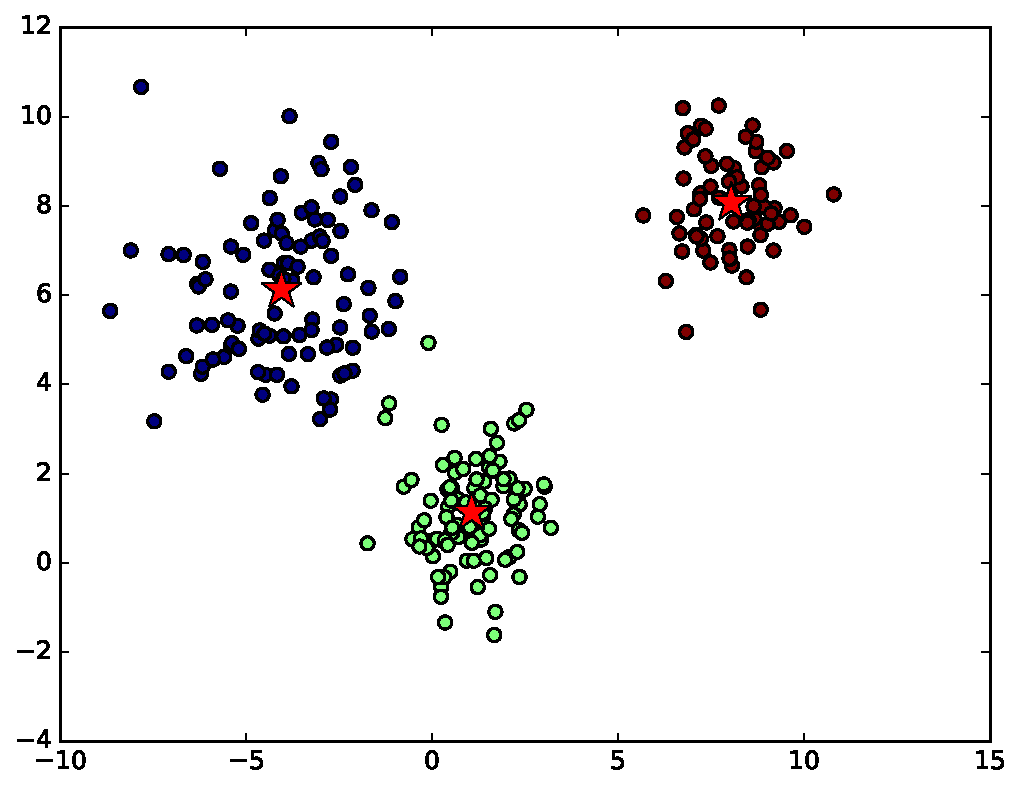
\includegraphics[width=0.25\textwidth]{img/kmeans/it08.pdf}\\
%\small{it 5} & \small{it 6} & \small{it 7} & \small{it 8}
%\end{tabular}
%\end{figure}
%\end{frame}
%\egroup

\begin{frame}{K-means: iterations}
\begin{center}
\animategraphics[loop,controls,width=0.5\textwidth]{2}{img/kmeans/it}{01}{08}
\end{center}
\end{frame}

\begin{frame}{Application: color segmentation}
K-means can be employed for image segmentation, simply by grouping pixels in the color space. You can also add coordinates to each pixel to obtain a smooth output.
\begin{figure}
\begin{tabular}{cc}
\small{Image} & \small{Segmentation}\\
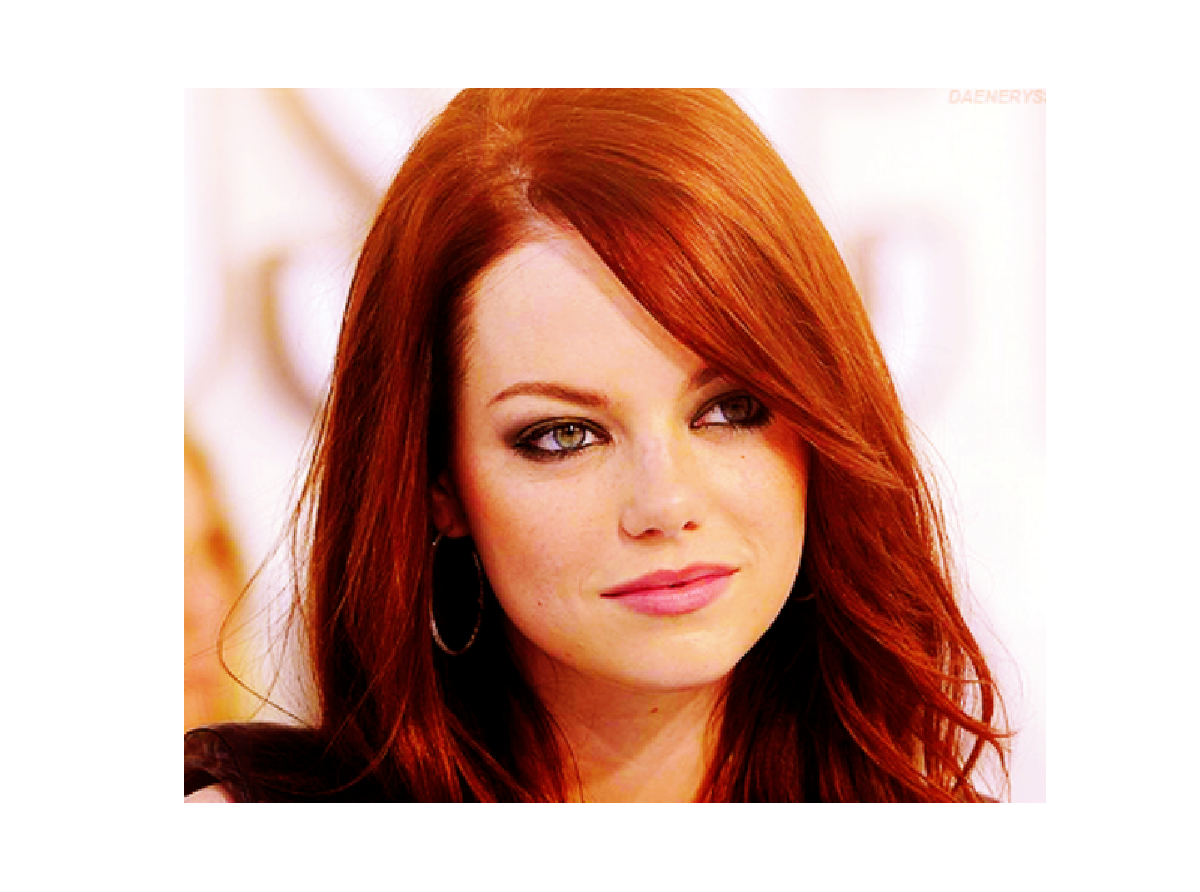
\includegraphics[width=0.35\textwidth]{img/kmeans/emma.pdf}&
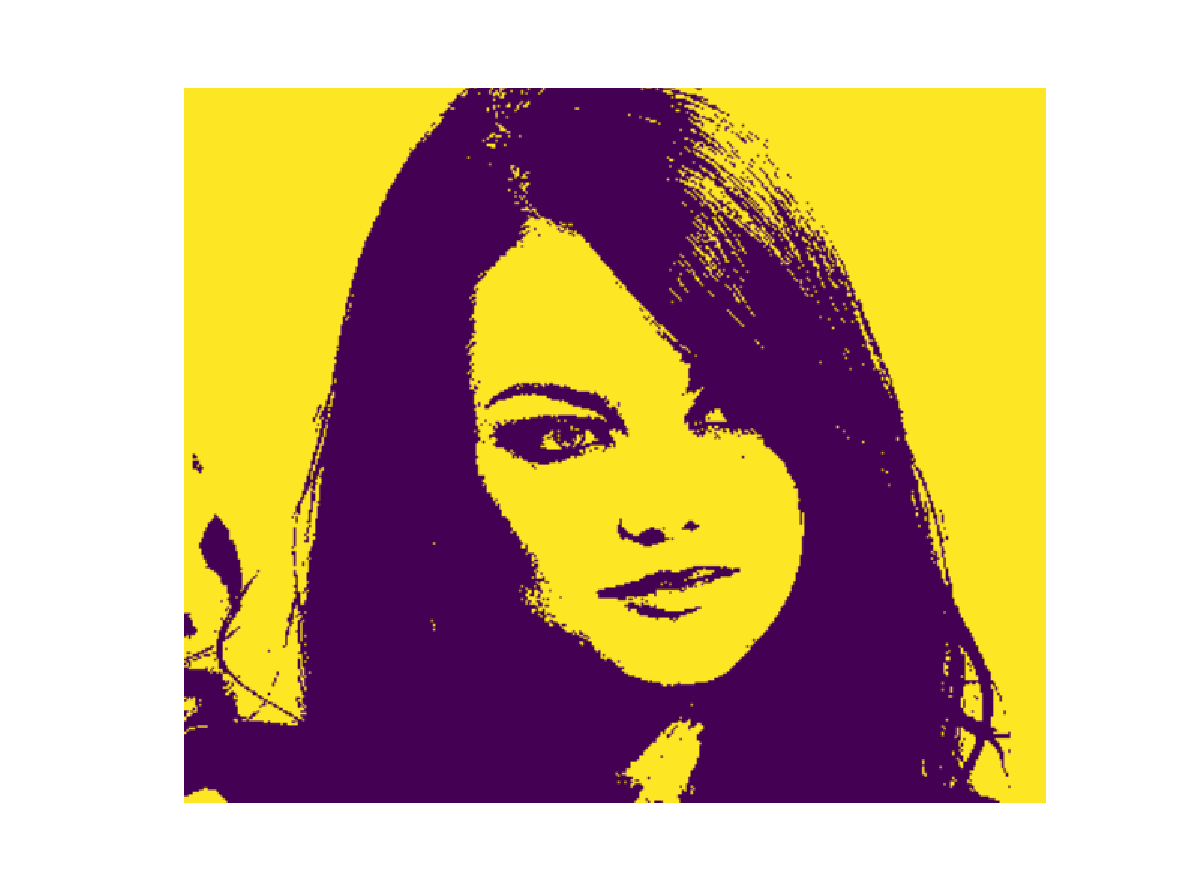
\includegraphics[width=0.35\textwidth]{img/kmeans/emma_segm.pdf}
\end{tabular}
\end{figure}
Try it!
\end{frame}
\begin{frame}{Kmeans: limitations}
\begin{itemize}
\item it can get stuck into bad local minima
\begin{itemize}
\item OPTIONAL: run the algorithm many times and choose the most recurrent solution
\end{itemize}
\item can only be employed in spaces where the mean operation is defined
\item due to its cost function, it can only cope with compact ball-shaped clusters
\begin{figure}
\begin{tabular}{cc}
\small{GT} & \small{Result}\\
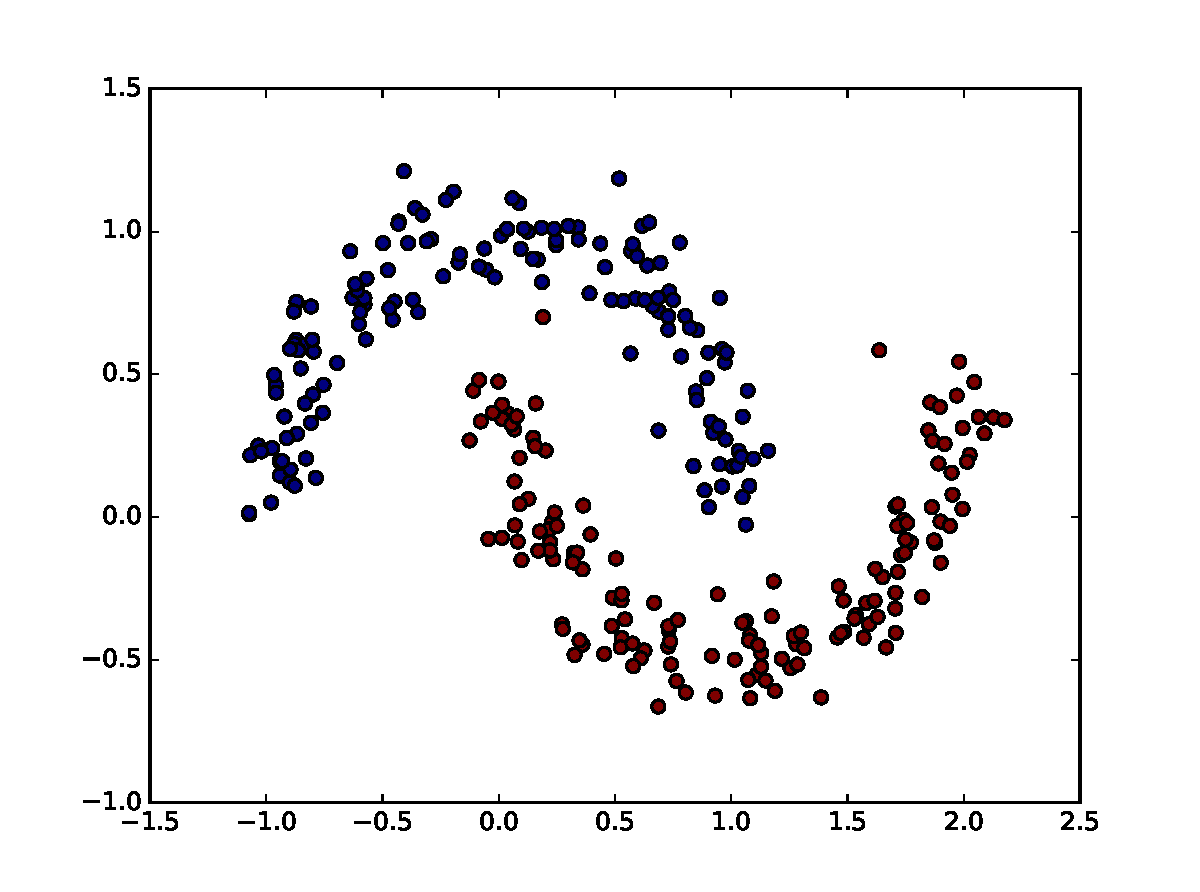
\includegraphics[width=0.35\textwidth]{img/kmeans/tm_gt.pdf}&
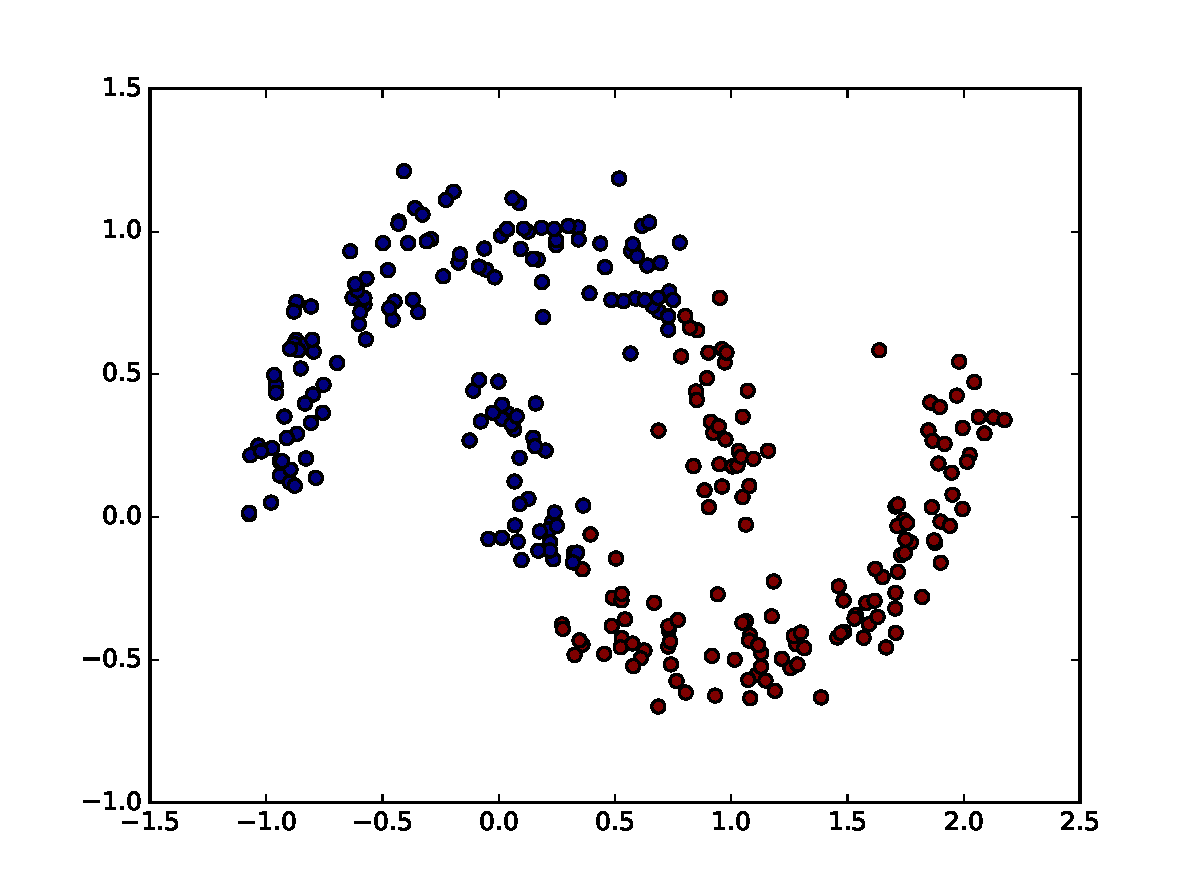
\includegraphics[width=0.35\textwidth]{img/kmeans/tm_fail.pdf}
\end{tabular}
\end{figure}
\end{itemize}
\end{frame}

\section{Spectral clustering}
\begin{frame}{Spectral clustering: algorithm (1)}
Clustering model based on the spectral graph theory.
\begin{itemize}
\item build a graph over examples, representing it with the adjacency matrix $A$
\begin{equation*}
A_{i,j} = e^{-\frac{\sum_{k=1}^d||x_i^k-x_j^k||^2}{\sigma^2}}
\end{equation*}
\item build the degree matrix $D$ of the graph. It is a diagonal matrix holding for each element the sum of the incoming adges.
\item compute the normalized laplacian $L$
\begin{equation}
L=I-D^{-0.5}AD^{-0.5}
\end{equation}
\end{itemize}
\end{frame}
\begin{frame}{Spectral clustering: algorithm (2)}
\begin{itemize}
\item Compute the eigenvectors and sort them for increasing eigenvalues
\item Choose the eigenvectors \underline{from the second to the desired number of clusters}
\item Those eigenvectors provide a representation of data in a fancy embedding space: run K-means over such eigenvectors.
\end{itemize}
\end{frame}
\bgroup
\begin{frame}{Spectral clustering: result}
\setlength{\tabcolsep}{.07em}
\begin{figure}
\begin{tabular}{cc}
\small{GT} & \small{Result}\\
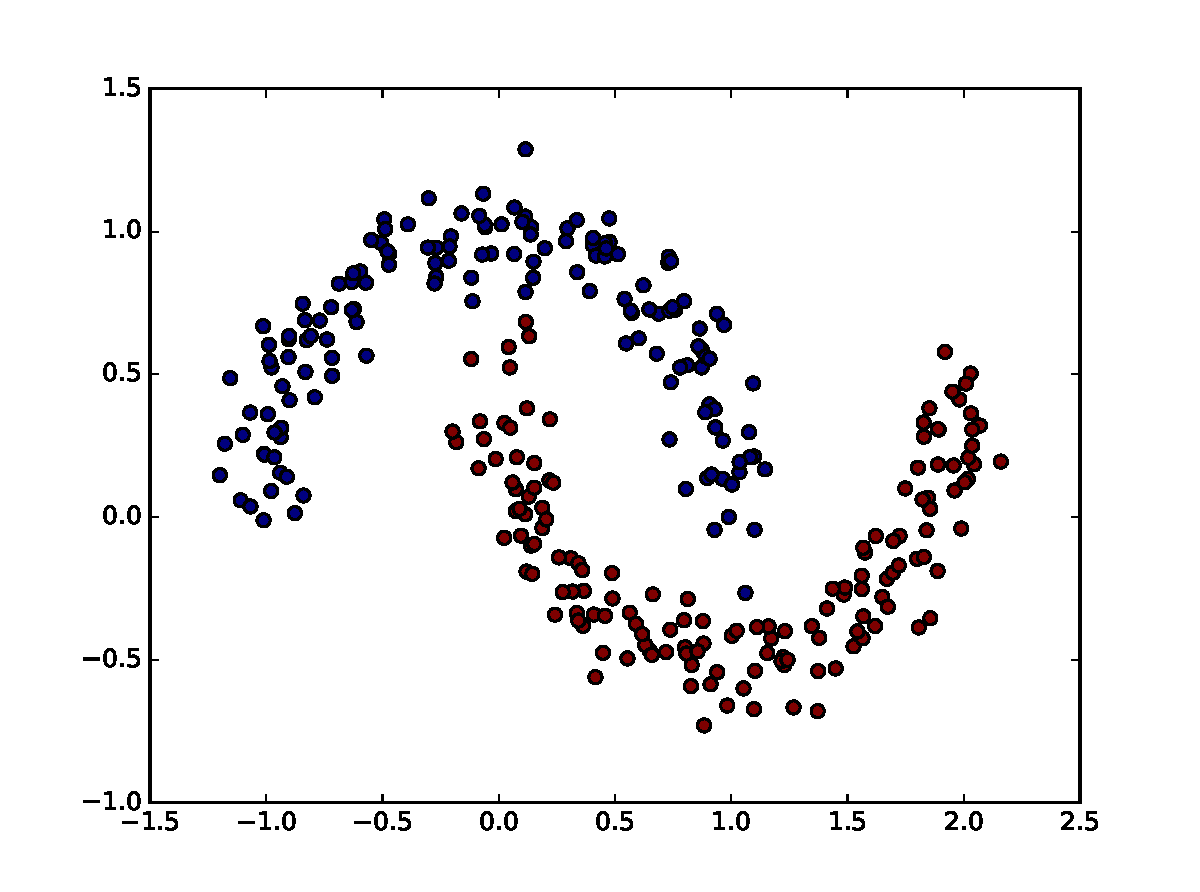
\includegraphics[width=0.45\textwidth]{img/spectral/gt.pdf}&
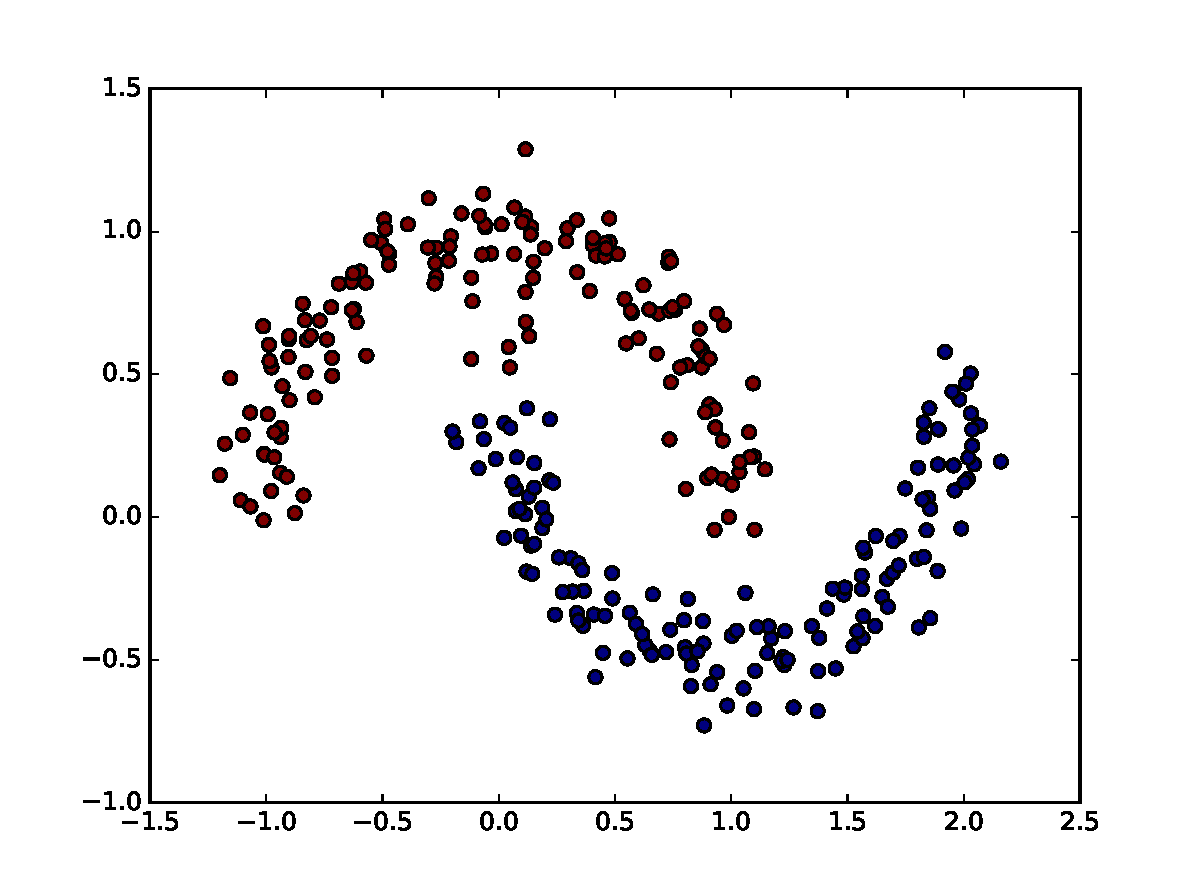
\includegraphics[width=0.45\textwidth]{img/spectral/pred.pdf}
\end{tabular}
\end{figure}
\end{frame}
\egroup
\bgroup
\begin{frame}{Beware: $\sigma$ counts (in large amounts!)}
\setlength{\tabcolsep}{.07em}
\begin{figure}
\begin{tabular}{ccc}
\small{$\sigma=0.01$} & \small{$\sigma=0.1$} & \small{$\sigma=1$}\\
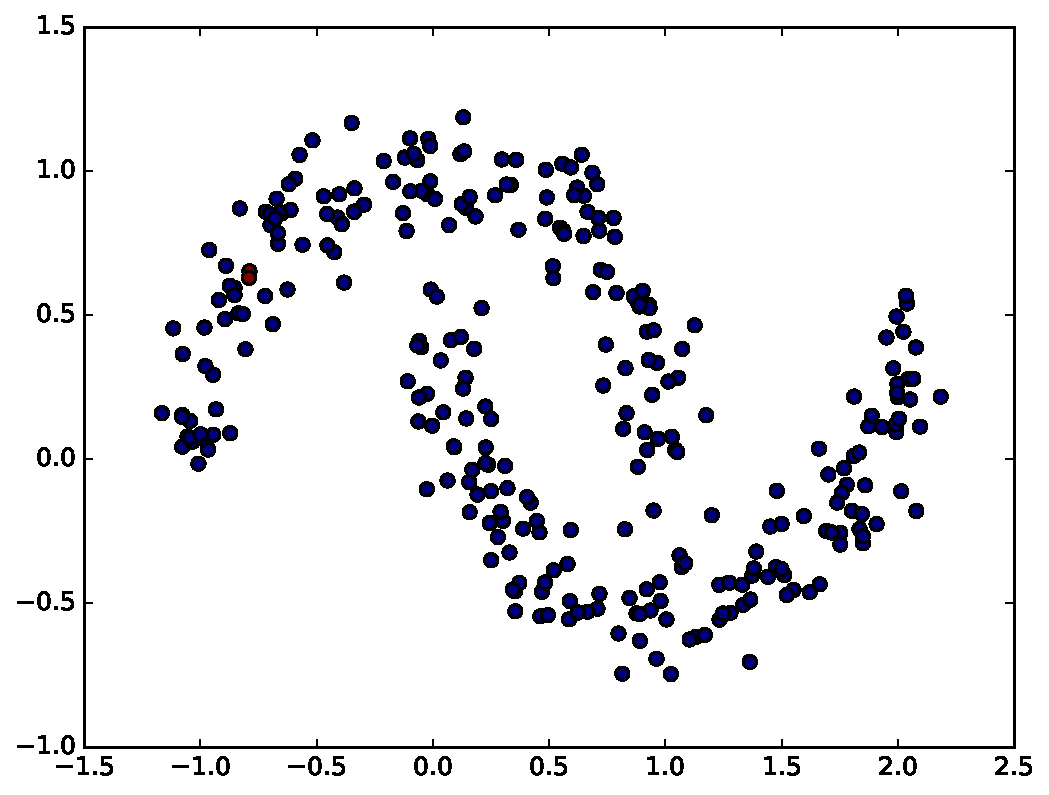
\includegraphics[width=0.3\textwidth]{img/spectral/sigma_0.pdf}&
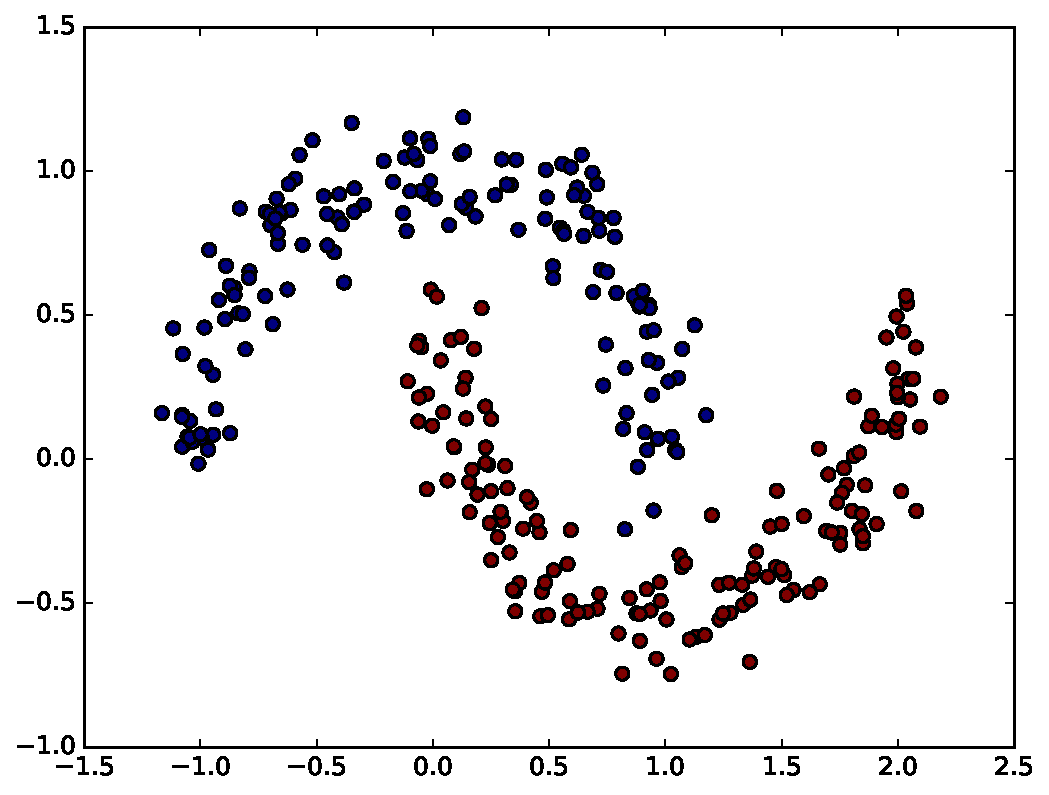
\includegraphics[width=0.3\textwidth]{img/spectral/sigma_2.pdf}&
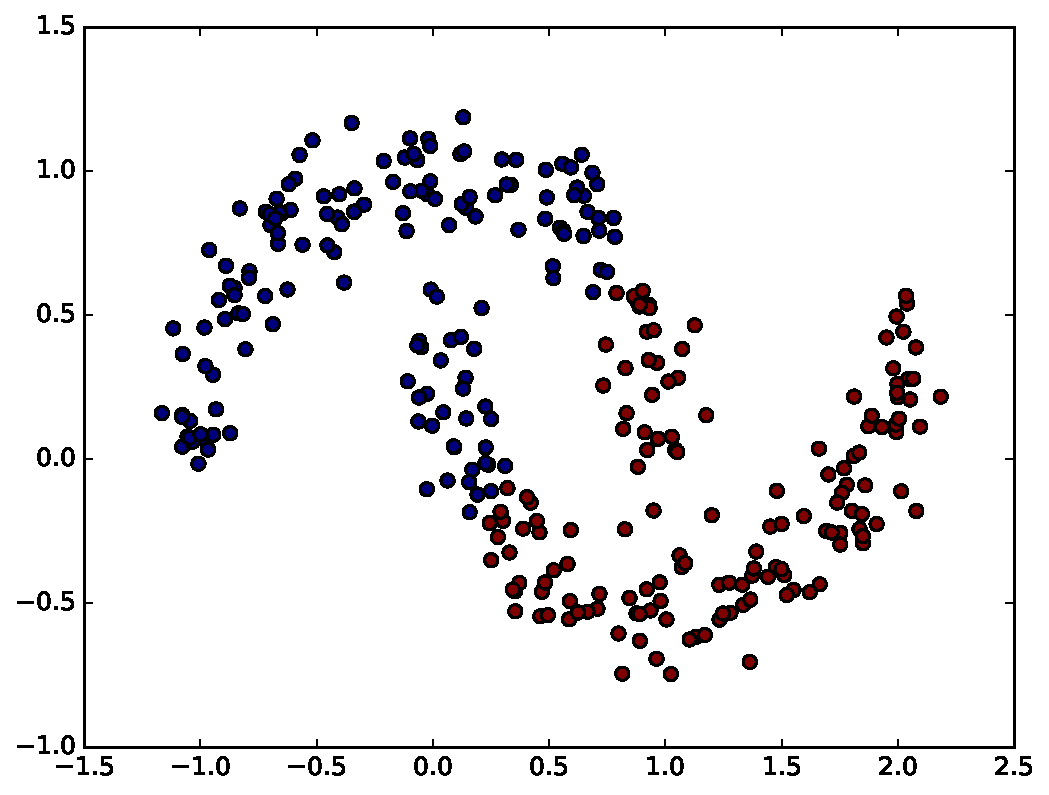
\includegraphics[width=0.3\textwidth]{img/spectral/sigma_4.pdf}
\end{tabular}
\end{figure}
\end{frame}
\egroup
\begin{frame}[fragile]{Useful functions}
\begin{itemize}
\item datasets.gaussian\_dataset
\begin{lstlisting}[frame=single, language=Python,basicstyle=\tiny]    
data, cl = gaussians_dataset(3, [100,100,70], [[1, 1],[-4, 6],[8, 8]], [[1, 1],[3, 3],[1, 1]])
\end{lstlisting}
\item datasets.two\_moon\_dataset
\begin{lstlisting}[frame=single, language=Python,basicstyle=\tiny]    
data, cl = two_moon_dataset(n_samples=300, noise=0.1)
\end{lstlisting}
\item \href{https://matplotlib.org/api/pyplot_api.html#matplotlib.pyplot.plot}{matplotlib.pyplot.plot}
\item \href{https://matplotlib.org/api/pyplot_api.html#matplotlib.pyplot.scatter}{matplotlib.pyplot.scatter}
\item \href{https://docs.scipy.org/doc/scipy-0.15.1/reference/generated/scipy.linalg.fractional_matrix_power.html
}{scipy.linalg.fractional\_matrix\_power}
\item \href{https://docs.scipy.org/doc/numpy-1.12.0/reference/generated/numpy.linalg.eig.html
}{numpy.linalg.eig}
\item \href{https://docs.scipy.org/doc/numpy-1.11.0/reference/generated/numpy.argsort.html}{numpy.argsort}\end{itemize}
\end{frame}
\end{document}